%%%%%%%%%%%%%%%%%%%%% chapter.tex %%%%%%%%%%%%%%%%%%%%%%%%%%%%%%%%%
%
% sample chapter
%
% Use this file as a template for your own input.
%
%%%%%%%%%%%%%%%%%%%%%%%% Springer-Verlag %%%%%%%%%%%%%%%%%%%%%%%%%%
%\motto{Use the template \emph{chapter.tex} to style the various elements of your chapter content.}
\chapter{An Overview on ETSI’s and Wi-Fi’s LBT Mechanisms}
\label{sec:LBT-overview} % Always give a unique label
% use \chaptermark{}
% to alter or adjust the chapter heading in the running head
%
%\abstract*{Each chapter should be preceded by an abstract (10--15 lines long) that summarizes the content. The abstract will appear \textit{online} at \url{www.SpringerLink.com} and be available with unrestricted access. This allows unregistered users to read the abstract as a teaser for the complete chapter. As a general rule the abstracts will not appear in the printed version of your book unless it is the style of your particular book or that of the series to which your book belongs.
%Please use the 'starred' version of the new Springer \texttt{abstract} command for typesetting the text of the online abstracts (cf. source file of this chapter template \texttt{abstract}) and include them with the source files of your manuscript. Use the plain \texttt{abstract} command if the abstract is also to appear in the printed version of the book.}

%TODO: Abstract
\abstract{Each chapter should be preceded by an abstract (10--15 lines long) that summarizes the content. The abstract will appear \textit{online} at \url{www.SpringerLink.com} and be available with unrestricted access. This allows unregistered users to read the abstract as a teaser for the complete chapter. As a general rule the abstracts will not appear in the printed version of your book unless it is the style of your particular book or that of the series to which your book belongs.\newline\indent
Please use the 'starred' version of the new Springer \texttt{abstract} command for typesetting the text of the online abstracts (cf. source file of this chapter template \texttt{abstract}) and include them with the source files of your manuscript. Use the plain \texttt{abstract} command if the abstract is also to appear in the printed version of the book.}


\section{ETSI’s LBT Mechanisms}
\label{subsec:ETSI-LBT-overview}
In \cite{LBT-ETSI-2014}, ETSI describes a number of spectrum access requirements to facilitate spectrum sharing for wireless access systems in $5$ GHz frequency band. This subsections focuses on requirements related to LBT mechanisms by which an equipment or a device applies CCA before using the channel to avoid collisions. The first mechanism is Frame Based Equipment (FBE) which defines a fixed (not directly demand-driven) timing frame for channel access. The second mechanism is Load Based Equipment (LBE) which defines demand-driven timing frame.

\begin{figure}[!t]
	\centering
	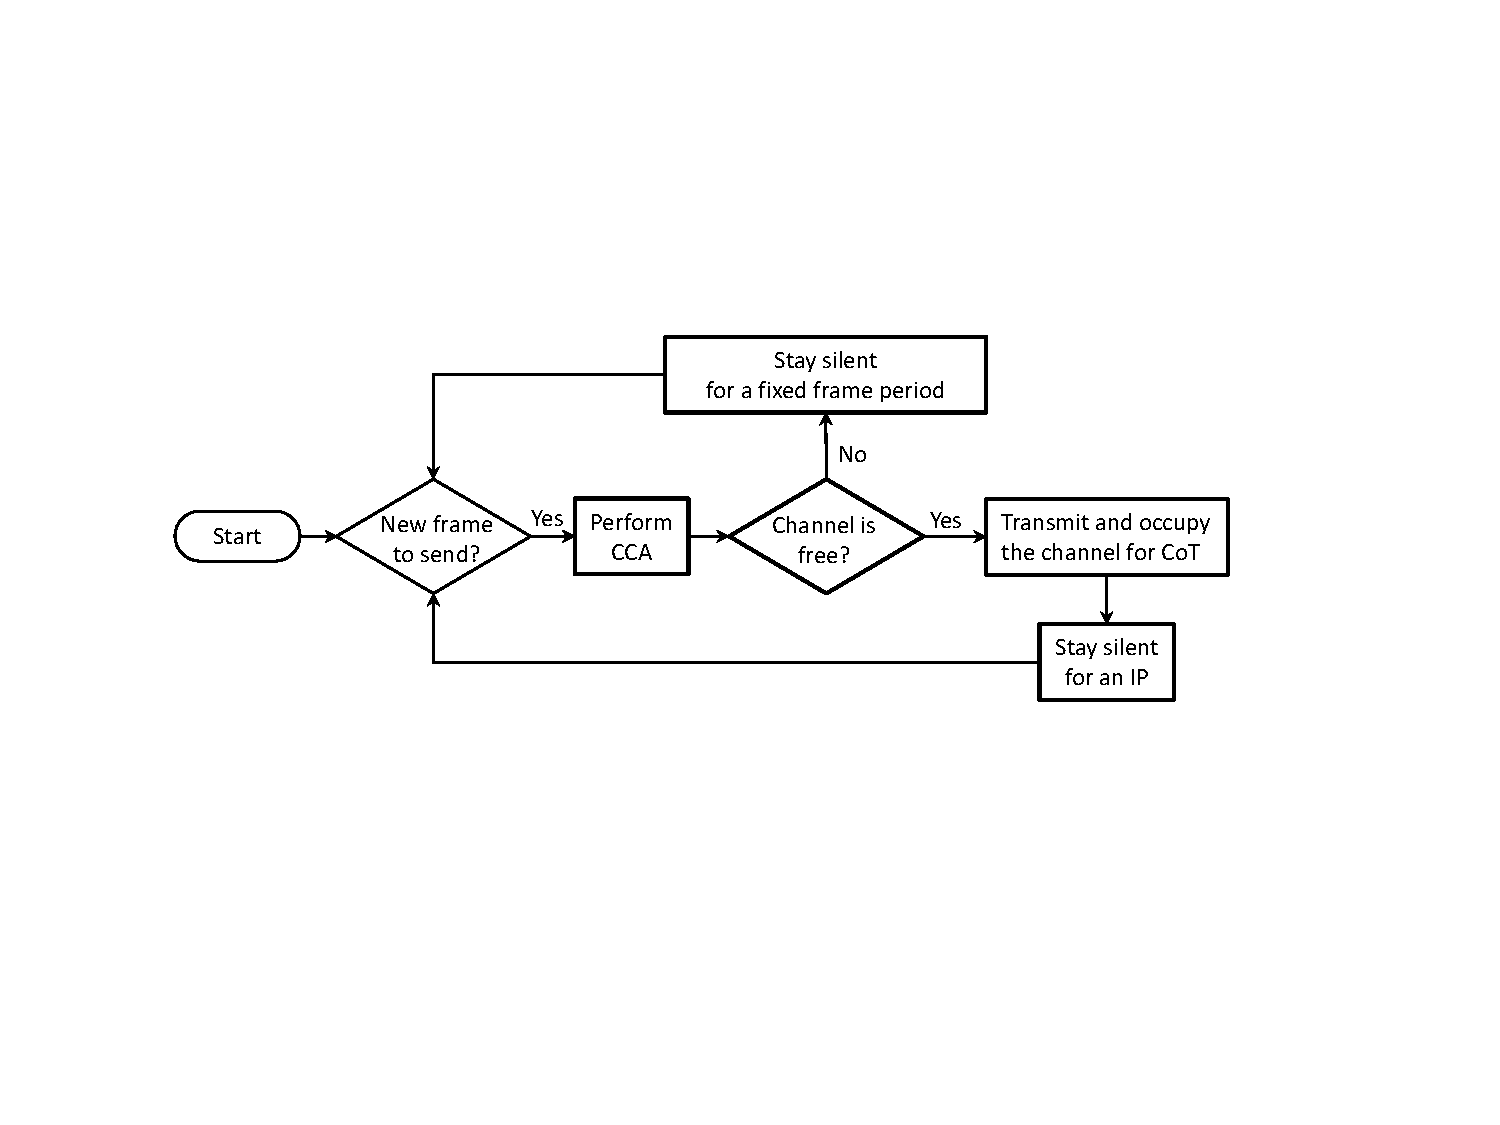
\includegraphics[width=0.9\columnwidth]{figures2/FBE-flowchart}
	\caption{Simplified flowchart of FBE.}
	\label{figs:FBE-flowchart}
\end{figure}

\begin{figure}[!t]
	\centering
	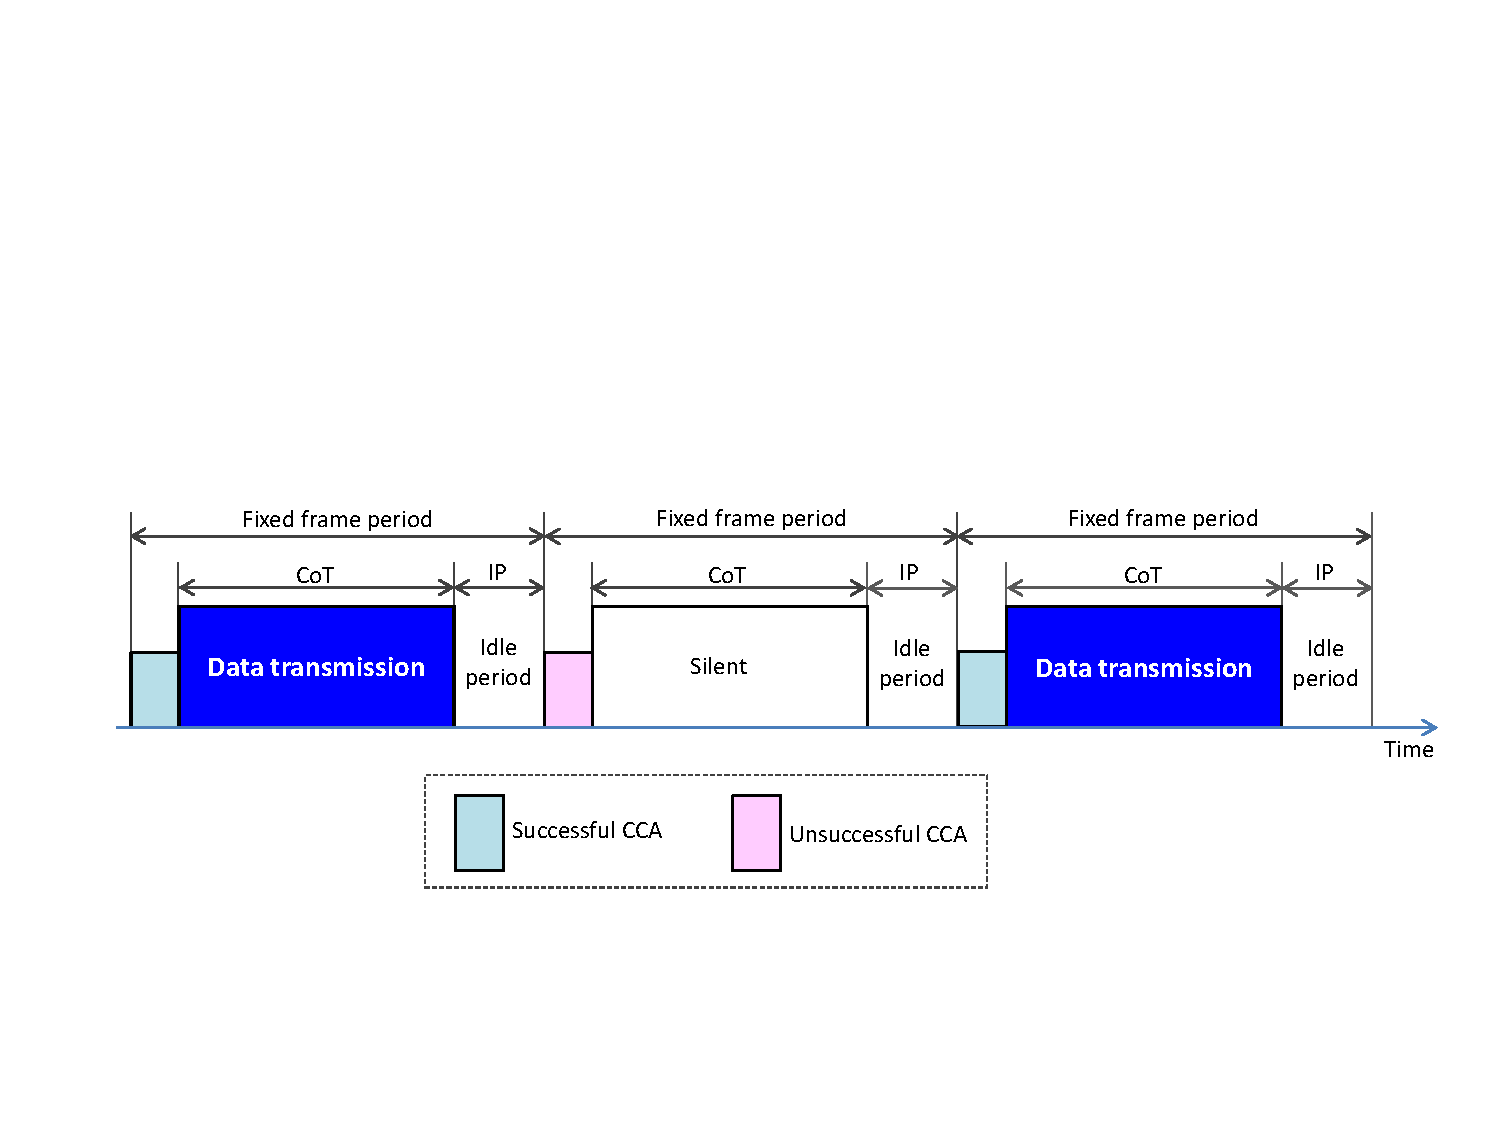
\includegraphics[width=0.9\columnwidth]{figures2/FBE-example}
	\caption{An illustrative example of FBE.}
	\label{figs:FBE-example}
\end{figure}

\subsection{FBE-based Mechanism}
\label{etsi-lbt:fbe}
FBE shall comply with the following requirements:

\begin{itemize}
	
	\item
	\textit{R1:} Before starting transmissions on an operating channel, the equipment shall perform a CCA check using Energy Detect (ED). The equipment shall observe the channel for the duration of the \textit{CCA observation time}. The operating channel shall be considered occupied if the energy level in the channel exceeds the \textit{threshold} corresponding to the power level.
	
	\item
	\textit{R2:}
	If the CCA procedure finds the channel clear, the equipment may transmit immediately and occupy the channel for a \textit{fixed time period}.
	
	\item
	\textit{R3:} If the CCA procedure finds the channel occupied, the equipment shall not transmit on that channel during the next fixed frame period.
	
	\item
	\textit{R4:} The total time during which an equipment has transmissions on a given channel without re-evaluating the availability of that channel is defined as the \textit{Channel Occupancy Time} (CoT).
	
	\item
	\textit{R5:} After occupying the channel for CoT, the equipment keeps silent and waits for a short time, namely \textit{Idle Period} (IP).
	
	\item
	\textit{R6:} Towards the end of the idle period, the equipment shall perform a new CCA procedure as described in R1 above.
	
	\item
	\textit{R7:} The equipment, upon correct reception of a packet which was intended for this equipment, can skip CCA and immediately proceed with the transmission of management and control frames, e.g., acknowledgment (ACK) and block ACK frames.
	
	\item
	\textit{R8:}
	A consecutive sequence of such transmissions by the equipment, without it performing a new CCA, shall not exceed the maximum CoT.
	
	\item
	\textit{R9:}
	CCA observation time shall be not less than $20$ $\mu$s.
	
	\item
	\textit{R10:} CoT shall be in the range from $1$ ms to $10$ ms.
	
	\item
	\textit{R11:}
	The minimum IP shall be at least $5$\% of CoT used by the equipment for the current fixed frame period.
	
\end{itemize}

A simplified flowchart and an illustrative of FBE are given in Figs. \ref{figs:FBE-flowchart} and \ref{figs:FBE-example}, respectively.


\begin{figure}[!t]
	\centering
	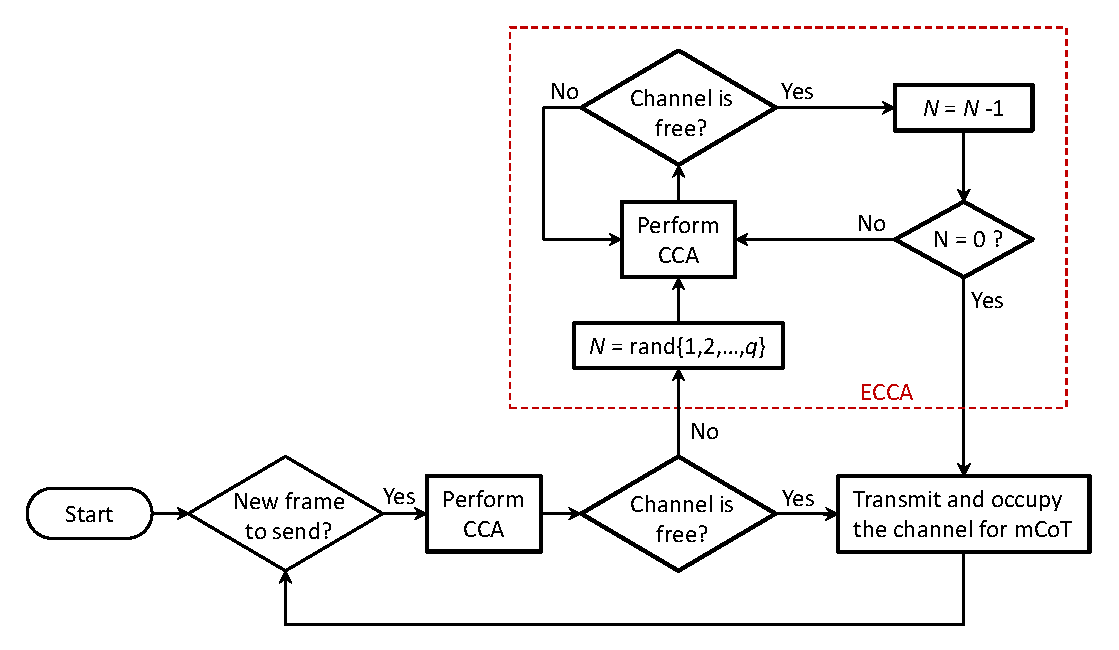
\includegraphics[width=0.9\columnwidth]{figures2/LBE-flowchart}
	\caption{Simplified flowchart of LBE.}
	\label{figs:LBE-flowchart}
\end{figure}

\begin{figure}[!t]
	\centering
	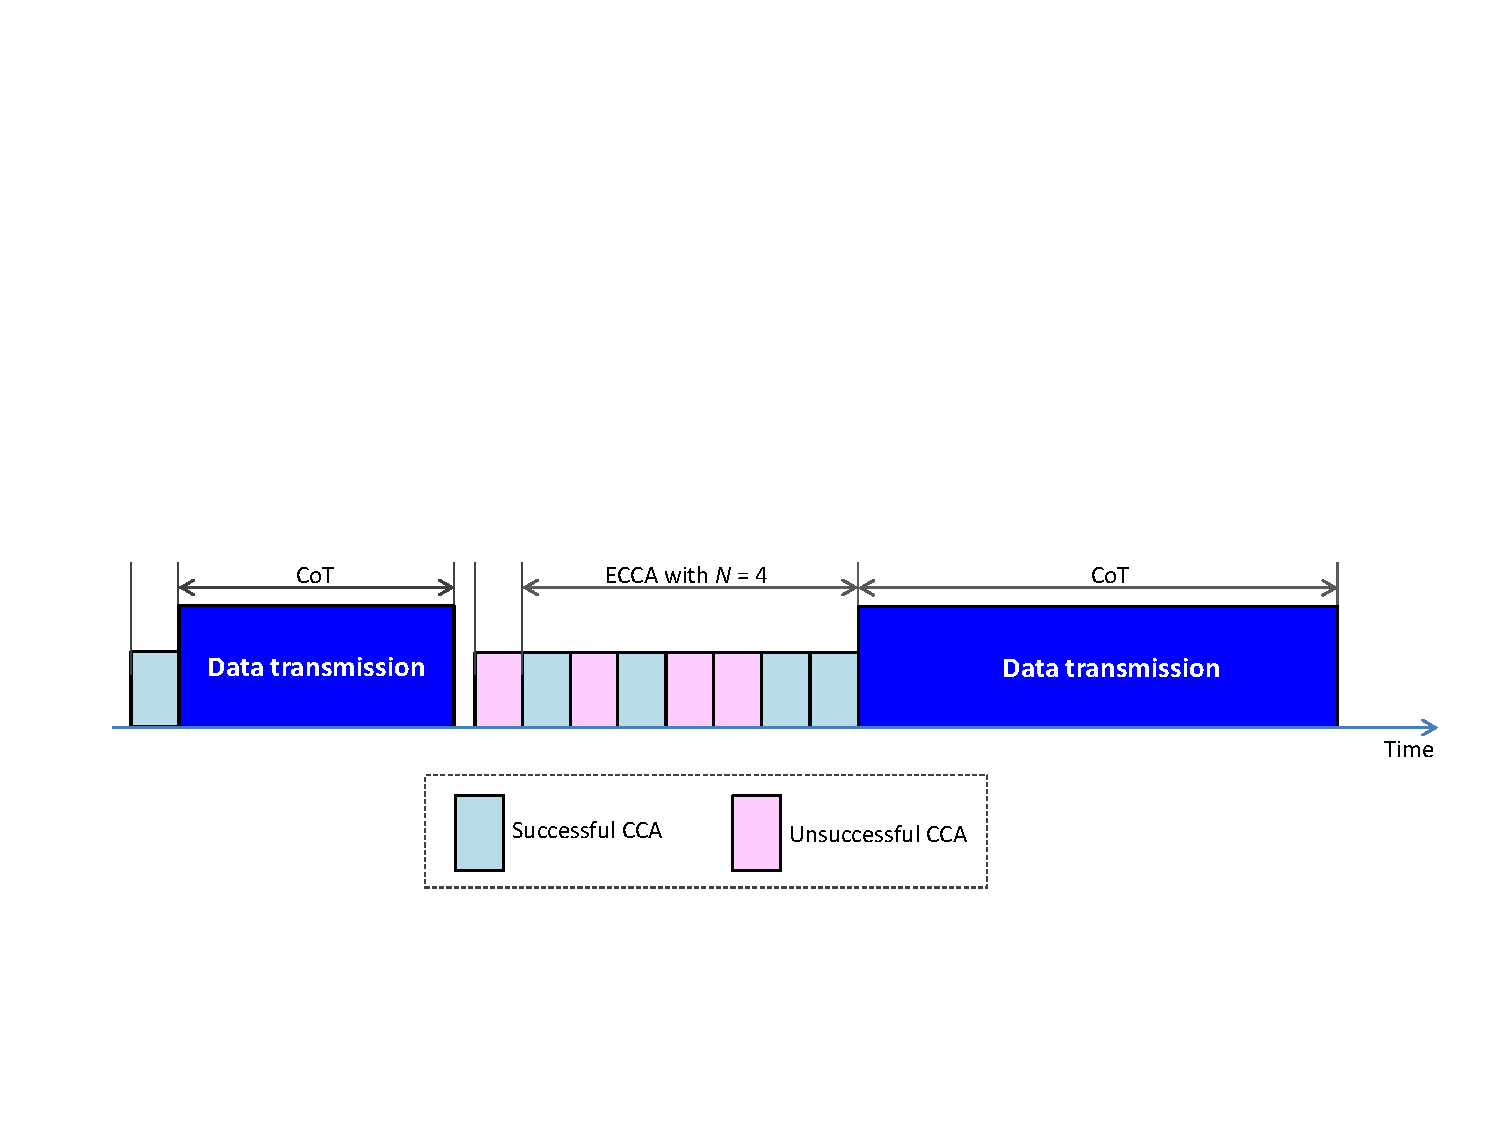
\includegraphics[width=0.9\columnwidth]{figures2/LBE-example}
	\caption{An illustrative example of LBE.}
	\label{figs:LBE-example}
\end{figure}

\subsection{LBE-based Mechanism}
\label{etsi-lbt:lbe}
LBE shall comply with the following requirements:

\begin{itemize}
	
	\item
	\textit{R1:} Before starting transmissions on an operating channel, the equipment shall perform a CCA check using ED. The equipment shall observe the channel for the duration of the \textit{CCA observation time}. The operating channel shall be considered occupied if the energy level in the channel exceeds the threshold corresponding to the power level.
	
	\item
	\textit{R2:}
	If the CCA procedure finds the channel clear, the equipment may transmit immediately on that channel.
	
	\item
	\textit{R3:}
	If the CCA procedure finds the channel occupied, it shall not transmit in that channel. The equipment shall perform an Extended CCA (ECCA) procedure in which the channel is observed for a random duration.
	
	\item
	\textit{R4:}
	If the ECCA procedure has determined the channel to be clear, the equipment may start transmissions on this channel.
	
	\item
	\textit{R5:}
	The total time that an equipment makes use of the channel (without performing CCA) is the \textit{maximum Channel Occupancy Time} (mCoT), after which the device shall perform a new CCA procedure as described in R1 above.
	
	\item
	\textit{R6:}
	The equipment, upon correct reception of a packet which was intended for this equipment, can skip CCA and immediately proceed with the transmission of management and control frames, e.g., ACK and block ACK frames.
	
	\item
	\textit{R7:}
	A consecutive sequence of transmissions by the equipment, without it performing a new CCA, shall not exceed mCoT.
	
	\item
	\textit{R8:}
	CCA observation time shall be not less than $20$ $\mu$s.
	
	\item
	\textit{R9:}
	The random duration in an ECCA procedure is $N \times$ (CCA observation time), where $N$ is randomly selected in the range $\{1,2,...,q\}$, $q \in \{4,5,...,32\}$ (declared by the manufacturer).
	
	\item
	\textit{R10:}
	mCoT should be less than $(13/32)\times q$ ms (mCoT is in the range from $1.625$ to $13$ ms).
	
\end{itemize}

A simplified flowchart and an illustrative of LBE are given in Figs. \ref{figs:LBE-flowchart} and \ref{figs:LBE-example}, respectively.

\section{Wi-Fi's LBT Mechanisms}
\label{wifi-lbt}
\begin{figure}[!t]
	\centering
	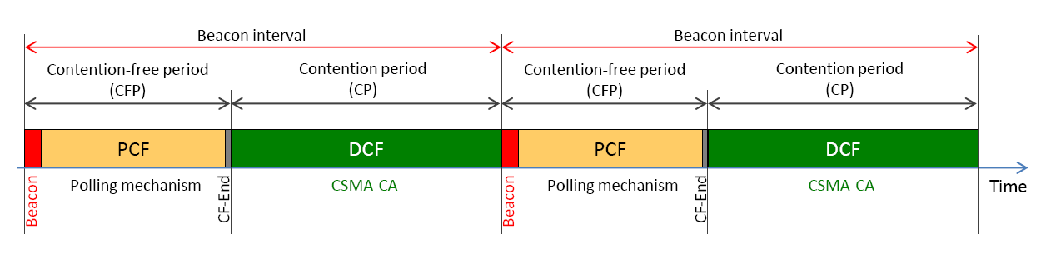
\includegraphics[width=1.0\columnwidth]{figures2/802-11-PCF-DCF}
	\caption{PCF and DCF in IEEE 802.11.}
	\label{figs:802-11-PCF-DCF}
\end{figure}

%%%%%%%%%%%%%%%%%%%%%%%% referenc.tex %%%%%%%%%%%%%%%%%%%%%%%%%%%%%%
% sample references
% %
% Use this file as a template for your own input.
%
%%%%%%%%%%%%%%%%%%%%%%%% Springer-Verlag %%%%%%%%%%%%%%%%%%%%%%%%%%

\begin{thebibliography}{99.}%
\bibitem{LBT-ETSI-2014}
\emph{ETSI EN 301 893 V1.7.2 (2014-07): Broadband Radio Access Networks (BRAN); 5 GHz high performance RLAN; Harmonized EN covering the essential requirements of article 3.2 of the R\&TTE Directive}, European Telecommunications Standards Institute Std., 2014.
\end{thebibliography}
